We consider a one dimensional spin chain from complete fixing
of the temporal links of a two dimensional gauge theory with action,
\begin{equation}
	S(U) = - \sum_x β \Real\tr [Uₓ^†Uₓ₊₁].
\end{equation}
With $U(1)$ gauge group, we use phase angle, $θ∈[-π,π)$, and
\begin{align}
	U &= e^{iθ}, \\
	S(U) &= - \sum_x β \cos[θₓ₊₁-θₓ],
\end{align}
which is a one dimensional $O(2)$ model.
With open boundary conditions, we can perform a
change of variable for a chain of $N$ spins,
\begin{equation}
	φₓ = θₓ₊₁-θₓ,
\end{equation}
\begin{align}
	Z &= \int \dd θ \prod_x e^{β \cos[θₓ₊₁-θₓ]} \\
	&= \int \dd φ \prod_x e^{β \cos[φₓ]} \\
	&= \prod_x ∫_{-\pi}^\pi \dd φ e^{β \cos φ},
\end{align}
where all the spins decouple.
This gives us the expectation value of the plaquette,
exactly the same as for the 2D $U(1)$ gauge theory in the limit,
\begin{equation}
	\langle P\rangle = \frac{I_1(\beta)}{I_0(\beta)},
\end{equation}
where $I$ is the modified Bessel function of the first kind,
\begin{align}
	I_n(z)
	&= \frac{1}{2\pi i}
		\oint e^{(t+1/t)z/2} t^{-n-1} dt \\
	&= \frac{1}{\pi}
		\int_0^\pi e^{z \cos\theta} \cos(n\theta) d\theta
		\quad\text{for } n\in \mathbb{Z}.
\end{align}

We can define the topological charge the same
as in the 2D U(1) model,
\begin{equation}
	Q = \frac{1}{2\pi} \sum_x \Arg [θₓ₊₁-θₓ].
\end{equation}

For the field transformation, we use
``stout smearing''~\cite{Morningstar:2003gk} style update,
which is also used in the perturbative treatment in reference~\cite{Luscher:2009eq}.
Given the 1D analogy of $n$ cycle Wilson loops of length $d$,
\begin{equation}
	W_{ndx}^{\text{even/odd}}(θ) = -\frac{γ_{nd}^{\text{even/odd}}}{n²} \cos\left[n(θ_{x+d}-θₓ)\right],
\end{equation}
our smearing update from $θ$ to $θ'$ is
\begin{equation}
	θ'_x = F_{ndx}^{\text{even/odd}}(θ) = θₓ + \frac{∂}{∂θₓ}W_{ndy}^{\text{even/odd}}(θ).
\end{equation}
In order to have a tractable Jacobian determinant,
we update ``even'' and ``odd'' sites separately,
\begin{align}
	\text{even: } & x \mod 2d <d, \\
	\text{odd: }  & x \mod 2d ≥d.
\end{align}
This defines a series of diffeomorphism with positive definite
Jacobian determinant with
\begin{equation}
	-0.5 < γ < 0.5.
\end{equation}

We optimize the coefficients, $γ$, during HMC,
by minimize the loss function defined as,
\begin{equation}
\begin{split}
	l(θ',π'|θ,π) &= - \frac{1}{N_{\text{batch}}} \sum_{\text{batch}}
	\max\left\{1, e^{H(θ,π)-H(θ',π')}\right\} \\
	&\Bigg(
		λ \frac{1}{N} \sum_x \left[ 1-\cos\left((θ'ₓ₊₁-θ'ₓ)-(θₓ₊₁-θₓ)\right) \right] \\
		&+ μ \left[ \sum_x \sin(θ'ₓ₊₁-θ'ₓ)-\sum_x \sin(θₓ₊₁-θₓ) \right]²
	\Bigg),
\end{split}
\end{equation}
where $(θ',π')$ and $(θ,π)$ are respectively the proposed and initial configuration
in the MD evolution,
and the sum of $\sin$ is an approximate of the topological charge.

In the following test, we apply a chain of 48 transformations twice,
\begin{equation}
	F_{ndx}^{\text{odd}} \circ F_{ndx}^{\text{even}} \circ \cdot\cdot\cdot,
\end{equation}
with $n∈[1,2,3,4]$ and $d∈[1,2,4,8,16,32]$.
There are 96 free parameters, $γ$, in total.
In addition we also train the leapfrog step size.
We train these 97 parameters during HMC with changing $β$
from small to large in steps,
everytime allow thermolizating after changing $β$ before starting optimization.
We train the model on a system with the number of sites, $N=64$,
and apply the trained model to a system with the number of sites, $N=256$.

\begin{figure}
	\centering
	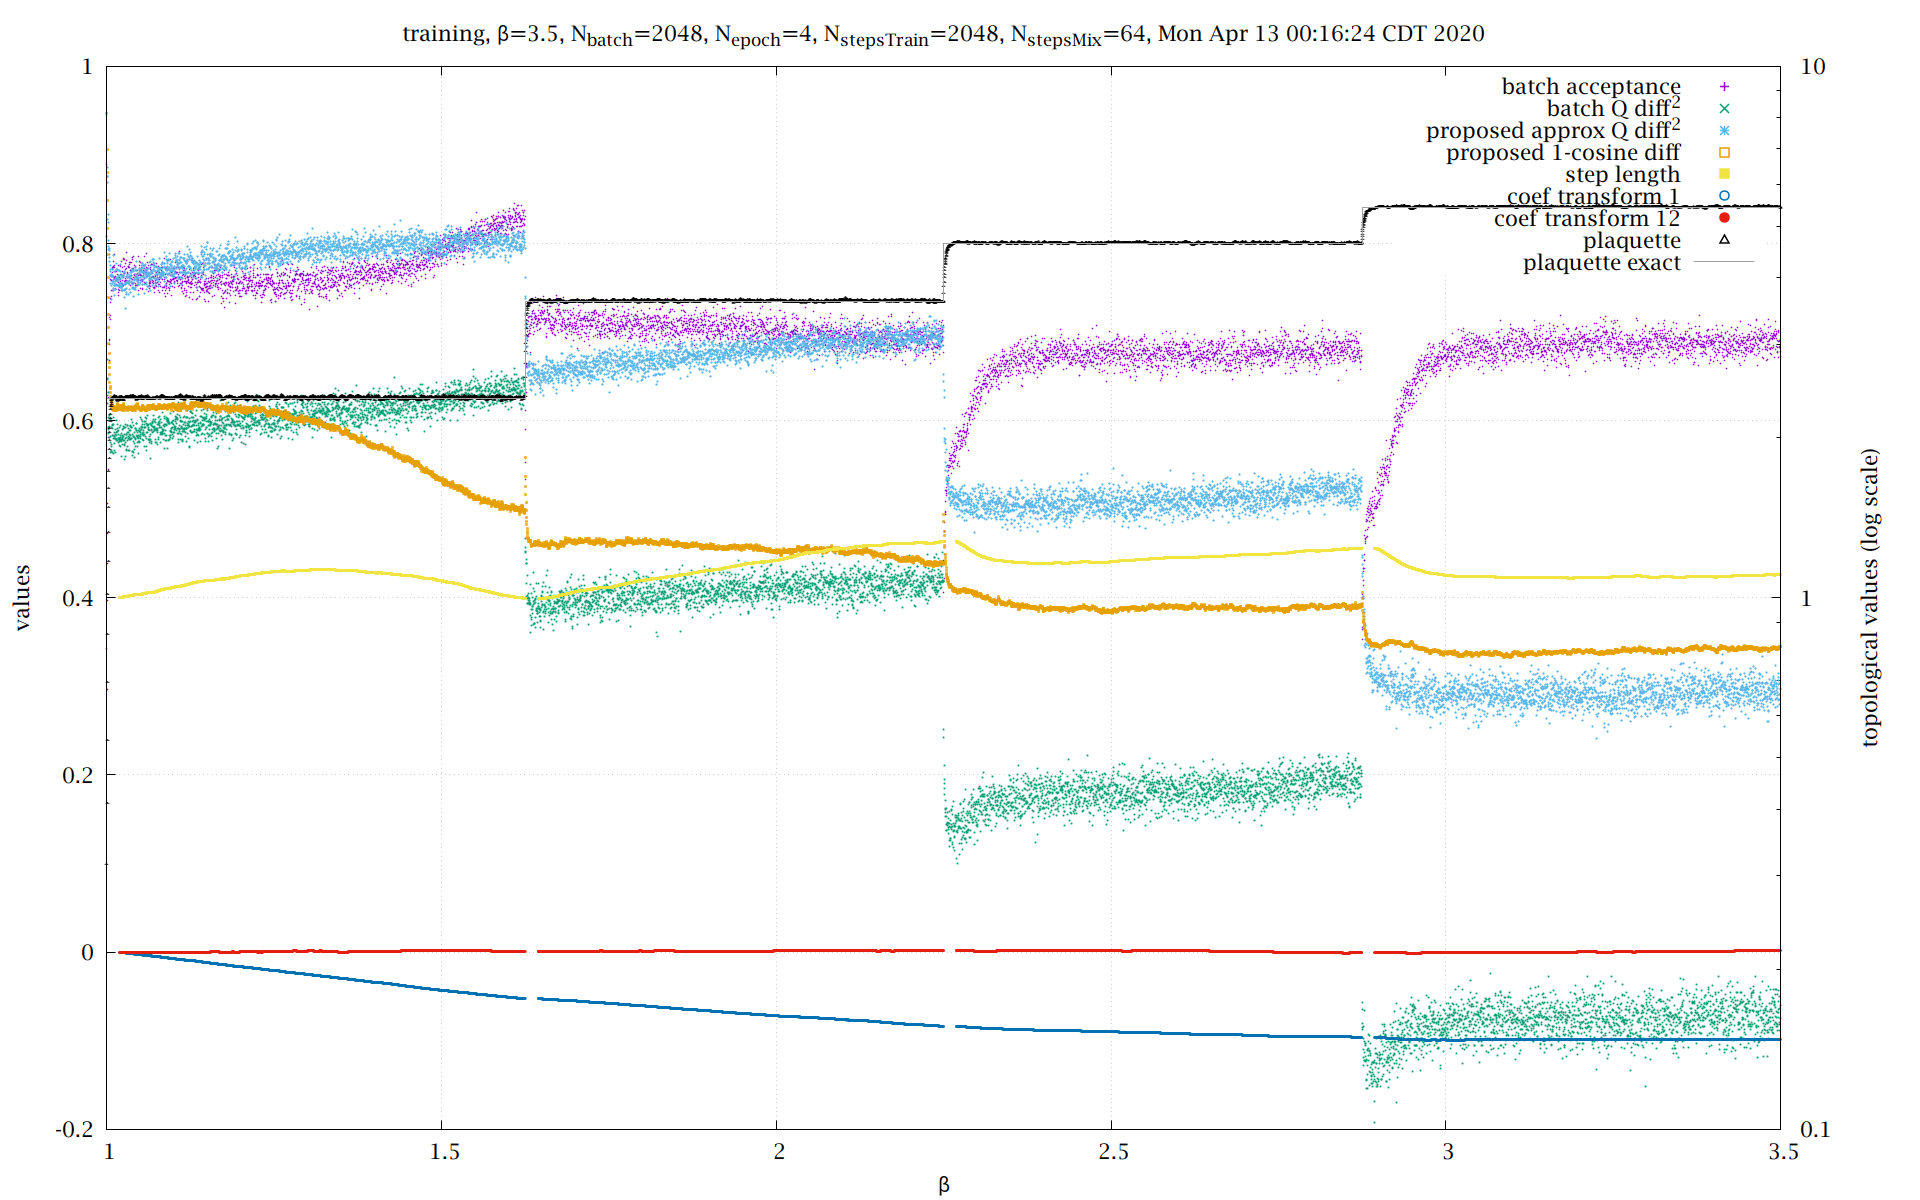
\includegraphics[width=\textwidth]{../t13.png}
	\caption{\label{training}Annealed training steps for $N=64$.}
\end{figure}

\begin{figure}
	\centering
	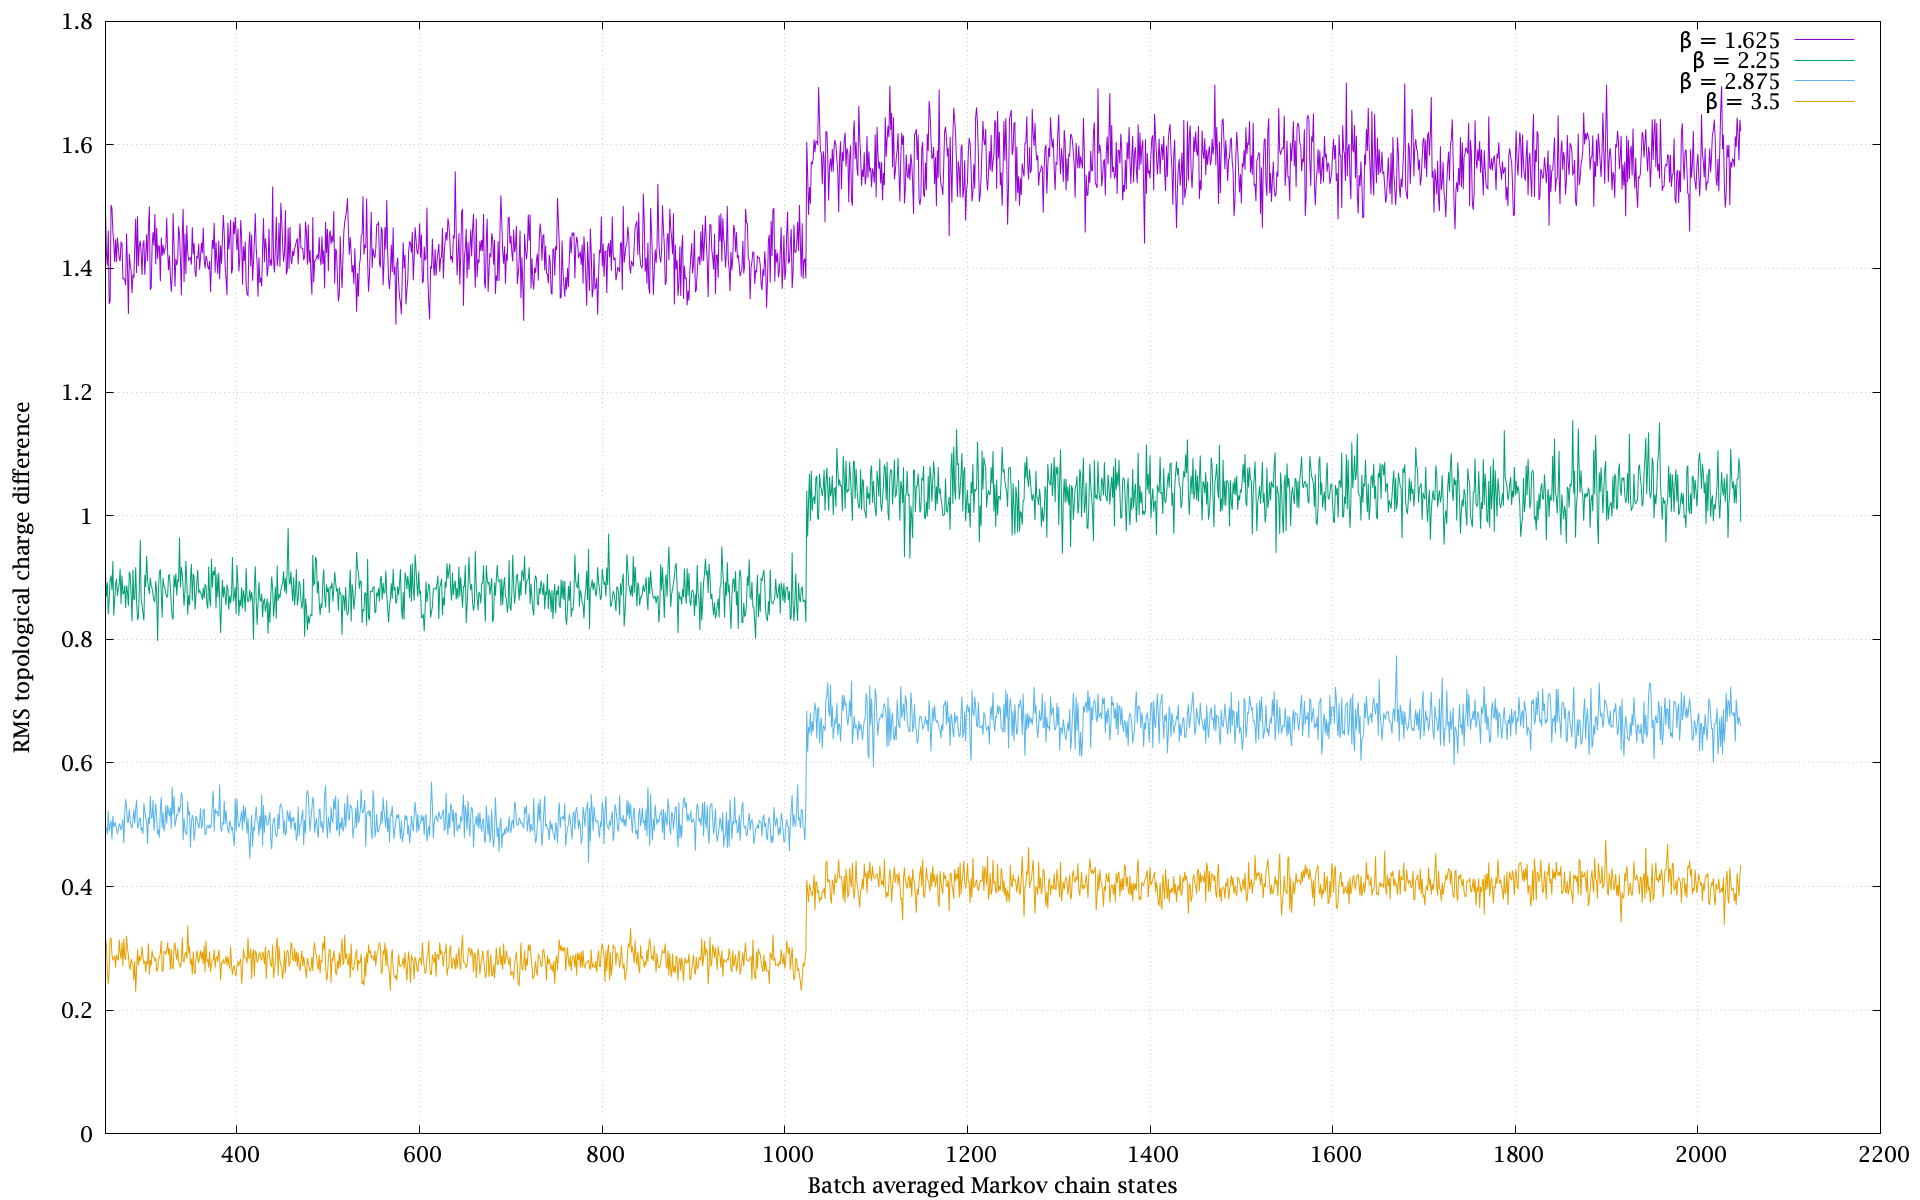
\includegraphics[width=\textwidth]{../topodiffN64.png}
	\caption{\label{topo-diff-n64}Topological charge change rate at $N=64$,
		with traditional HMC and field transformation HMC.}
\end{figure}

\begin{figure}
	\centering
	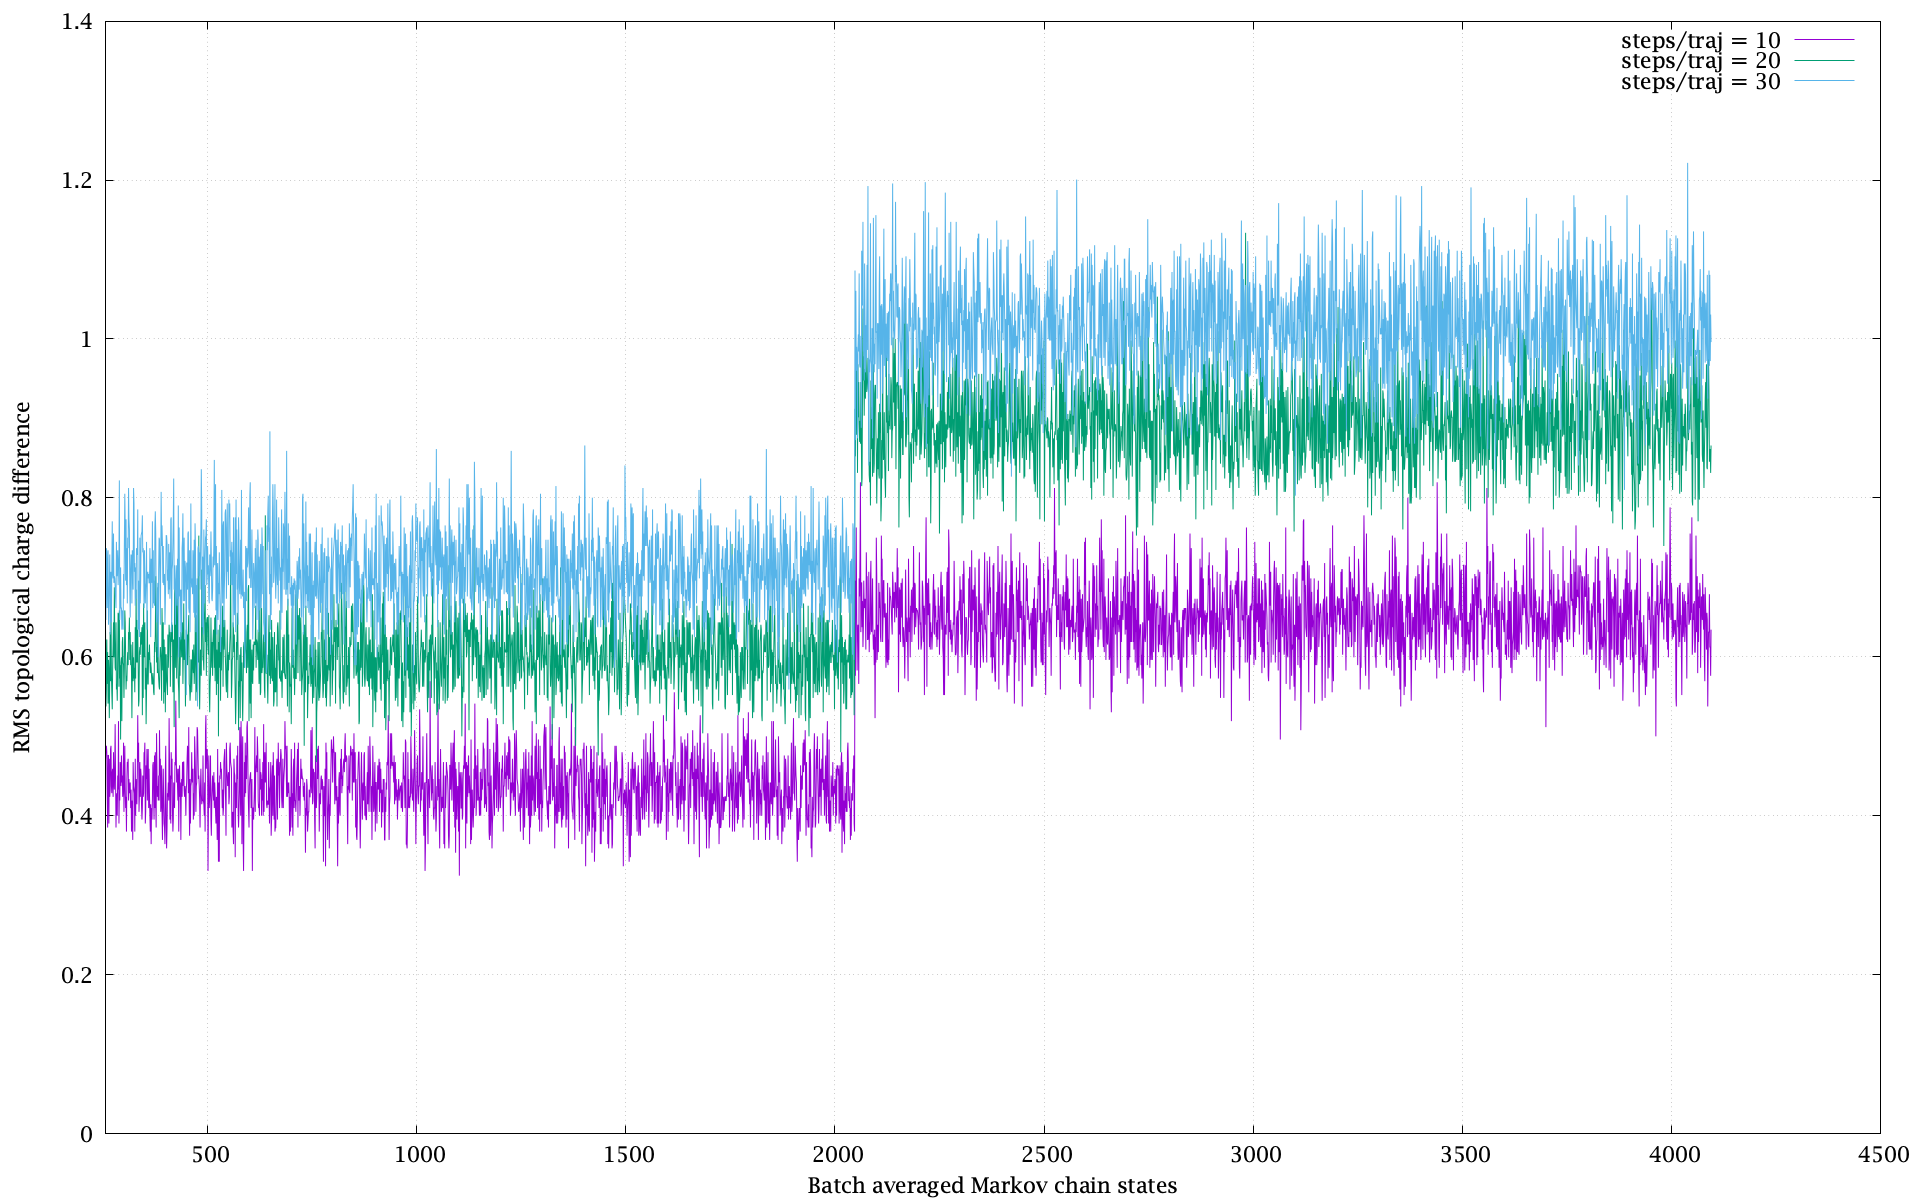
\includegraphics[width=\textwidth]{../topodiffN256.png}
	\caption{\label{topo-diff-n256}Apply trained parameters from $N=64$ to $N=256$,
		with traditional HMC and field transformation HMC.}
\end{figure}

\begin{figure}
	\centering
	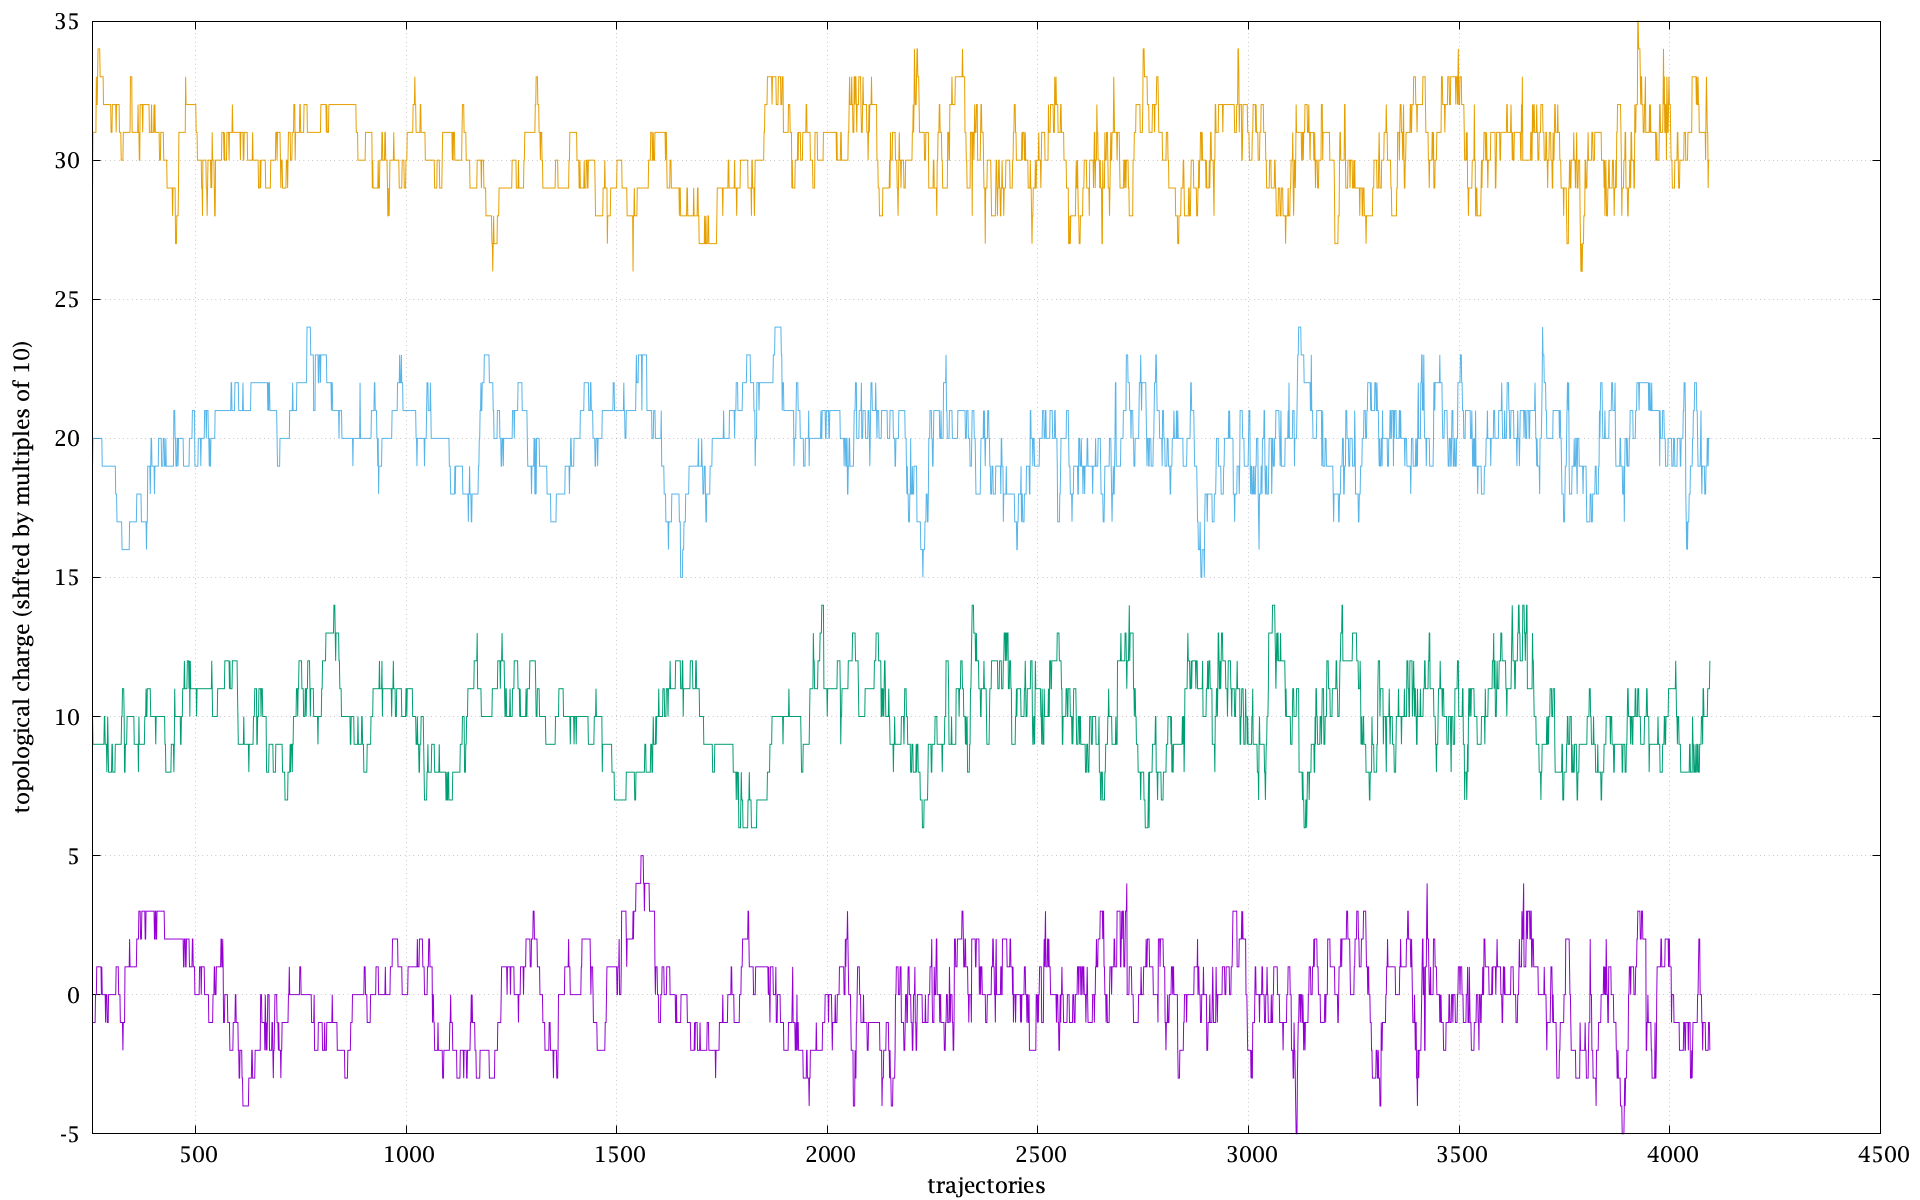
\includegraphics[width=\textwidth]{../topoevoN256.png}
	\caption{\label{topo-evo-n256}Individual MC evolution after
		applying trained parameters from $N=64$ to $N=256$,
		with traditional HMC and field transformation HMC.}
\end{figure}

